\documentclass[11pt,letterpaper]{article}
\usepackage{fontspec}
\setmainfont{DejaVu Serif}
\usepackage[spanish,es-noshorthands,es-tabla,es-nodecimaldot]{babel}
\usepackage[margin=2.5cm]{geometry}
\usepackage{amsmath}
\usepackage{graphicx,booktabs,array,float,caption,enumitem,setspace,xcolor,multicol}
\usepackage[hidelinks]{hyperref}
\usepackage{titlesec}
\titleformat{\section}{\large\bfseries}{\thesection.}{0.6em}{}
\titleformat{\subsection}{\normalsize\bfseries}{\thesubsection}{0.6em}{}
\captionsetup{font=small,labelfont=bf}
\setstretch{1.2}
\setlength{\parskip}{0.45em}
\setlength{\parindent}{0pt}
\graphicspath{{figs/}}
\newcommand{\pend}[1]{\textcolor{red}{#1}}

\begin{document}

\begin{center}
{\small Universidad de La Salle -- Facultad de Ingeniería -- Maestría en Inteligencia Artificial\par}
{\small Ciencia de Datos -- Proyecto Integrador, Informe Técnico Final\par}
\vspace{0.8cm}
{\LARGE\bfseries Predicción y caracterización de la inasistencia a citas médicas de consulta externa con aprendizaje automático\par}
\vspace{0.6cm}
{\large Jairo Teófilo Araméndiz Pinzón\par}
{\small Docente: Fabián Camilo Castro Riveros\par}
{\small Bogotá D.C., noviembre de 2026\par}
\end{center}

\vspace{0.4cm}
\noindent\rule{\textwidth}{0.4pt}

\textbf{Resumen.} La inasistencia a citas programadas deja cupos sin usar y alarga la espera de otros pacientes. Este trabajo analiza 110.527 citas de consulta externa de la red pública de Vitória (Brasil) para predecir qué citas terminarán en inasistencia, estimar los días de espera entre el agendamiento y la cita, y segmentar a los 62.299 pacientes según su patrón de uso. Se construyeron 11 variables derivadas, entre ellas el historial de inasistencias del paciente, y se usó una partición 70/15/15 estratificada y agrupada por paciente para evitar fuga de información. En clasificación, XGBoost obtuvo en el conjunto de prueba un AUC-ROC de 0,740, un F1 de 0,455 y detectó el 77,0\,\% de las inasistencias, frente a un AUC de 0,729 de la regresión logística de referencia; Random Forest y un perceptrón multicapa en PyTorch obtuvieron resultados equivalentes. La regresión de los días de espera alcanzó un $R^2$ de 0,138 con XGBoost, un valor bajo que se explica por la ausencia de variables de oferta (especialidad, profesional, agenda). K-Means con cinco segmentos identificó grupos interpretables, entre ellos dos con espera larga que se diferencian sobre todo por la cobertura de recordatorios SMS. El análisis SHAP mostró que, una vez se controla la espera, recibir un SMS se asocia con menor riesgo de inasistencia, lo que invierte la comparación directa. Los modelos se publicaron en un tablero interactivo con predicción en vivo, pensado como insumo para la política de recordatorios de un sistema conversacional de agendamiento médico.

\textbf{Palabras clave:} inasistencia a citas, \emph{no-show}, aprendizaje automático, XGBoost, SHAP, segmentación de pacientes, recordatorios SMS.

\noindent\rule{\textwidth}{0.4pt}

\section{Introducción}

Una cita a la que el paciente no asiste y que no cancela con anticipación es capacidad perdida: el profesional queda sin consulta en esa franja y el cupo no se puede reasignar. Dantas et al. (2018) revisaron 105 estudios sobre el tema y reportaron tasas de inasistencia muy variables según la región y el tipo de servicio, con un promedio cercano al 23\,\%. En la consulta externa colombiana el problema se cruza con las metas de oportunidad en la asignación de citas que fija la Resolución 1552 de 2013 del Ministerio de Salud y Protección Social.

Las revisiones de Van Buchem et al. (2022) y de Manarte y Guedes (2024) coinciden en que los sistemas digitales de agendamiento pueden mejorar la accesibilidad y reducir el ausentismo, y en que su efecto depende de cómo se integren a la operación. Una forma concreta de integración es usar un modelo predictivo para decidir a qué pacientes recordar o confirmar con más insistencia. Este proyecto se articula con el trabajo de grado del autor, AgendamientoIA, un sistema conversacional de agendamiento médico vía WhatsApp que envía recordatorios automáticos 24 horas antes de la cita.

Como el piloto de AgendamientoIA todavía no genera datos suficientes ni públicos, se usó el conjunto abierto \emph{Medical Appointment No Shows} (Hoppen, 2016), que según Salazar et al. (2022) es el más usado en la investigación sobre inasistencia. El trabajo responde a una pregunta principal: \emph{¿qué características del paciente y del proceso de agendamiento permiten anticipar la inasistencia a citas de consulta externa, y cómo pueden usarse esos patrones para priorizar recordatorios automáticos?} Las preguntas secundarias indagan por la relación entre la espera y la inasistencia controlando por el SMS, por los factores que explican la espera y por los perfiles de pacientes que se distinguen en los datos.

Los objetivos específicos fueron: (1) entrenar y comparar al menos dos clasificadores y obtener en prueba un AUC-ROC de al menos 0,70 y un F1 superior al del modelo base; (2) estimar los días de espera con una regresión regularizada y un ensamble de árboles, reportando $R^2$, RMSE y MAE; y (3) segmentar a los pacientes con K-Means y un segundo algoritmo, y publicar los resultados en un tablero interactivo.

\section{Metodología}

\subsection{Datos}
El conjunto contiene 110.527 citas de 62.299 pacientes, con 14 variables: identificadores, sexo, edad, barrio de la unidad de atención, fechas de agendamiento y de la cita, beneficio del programa Bolsa Família, hipertensión, diabetes, alcoholismo, número de discapacidades, recepción de SMS y la variable objetivo \emph{No-show}. Las citas van del 29 de abril al 8 de junio de 2016. La licencia es CC BY-NC-SA 4.0. El 20,19\,\% de las citas terminó en inasistencia.

\subsection{Limpieza y tratamiento de atípicos}
No hay celdas vacías, pero el análisis exploratorio encontró valores incoherentes. Se eliminaron 6 registros con eventos imposibles (una edad negativa y cinco citas anteriores a su agendamiento). Las cinco edades de 115 años, concentradas en dos pacientes, se trataron como faltantes después de analizar su origen: como el error viene de la ficha del paciente y no está repartido al azar entre citas, se descartó un mecanismo MCAR puro, y por el tamaño (0,005\,\%) se imputaron con la mediana de entrenamiento. Se conservaron los 1.275 grupos de registros con el mismo paciente, fecha e instante de agendamiento, porque en 29 de ellos el resultado difiere y no hay criterio objetivo para descartar uno de cada par. La cola larga de los días de espera (hasta 179) es real y concentra el mayor ausentismo, por lo que se recortó al percentil 99 aprendido en entrenamiento en lugar de eliminarla.

\subsection{Ingeniería de variables}
Se construyeron 11 variables con información disponible antes de la cita: días de espera, indicador de cita del mismo día, día de la semana de la cita y del agendamiento, hora del agendamiento, número de condiciones crónicas, grupo de edad, número de citas del paciente en la misma fecha, y el historial del paciente en fechas anteriores (citas previas, inasistencias previas y tasa de inasistencia previa). El 40,0\,\% de las citas tiene historial; la inasistencia pasa de 19,2\,\% en pacientes sin inasistencias previas a 32,1\,\% en quienes acumulan dos o más.

\subsection{Partición y preprocesamiento sin fuga de información}
Los datos se dividieron en entrenamiento (77.361 citas, 70,0\,\%), validación (16.577, 15,0\,\%) y prueba (16.583, 15,0\,\%) con \texttt{StratifiedGroupKFold}: la proporción de inasistencia se mantiene en 20,2\,\% en los tres conjuntos y ningún paciente aparece en más de uno. La imputación, la winsorización, el escalamiento (\texttt{StandardScaler}), la codificación \emph{one-hot} y la codificación por objetivo del barrio (\texttt{TargetEncoder}, 81 categorías) se ajustan solo con entrenamiento dentro de \emph{pipelines} de scikit-learn. Para la regresión de la espera se excluyeron el SMS, el indicador de cita del mismo día, el día de la cita y el mes de agendamiento, porque revelan el valor que se quiere predecir.

\subsection{Modelos y evaluación}
\textbf{Clasificación.} La referencia fue una regresión logística con \texttt{class\_weight='balanced'}. Se entrenaron Random Forest y XGBoost con búsqueda aleatoria de hiperparámetros (\texttt{RandomizedSearchCV}, 8 y 15 combinaciones) y validación cruzada de tres particiones estratificadas y agrupadas por paciente dentro de entrenamiento, con AUC-ROC como métrica. El desbalance de 4 a 1 se trató con ponderación de clases (\texttt{balanced\_subsample} y \texttt{scale\_pos\_weight}). Se agregó un perceptrón multicapa en PyTorch (35 → 64 → 32 → 1, ReLU, \emph{batch normalization}, \emph{dropout} de 0,3, pérdida BCE ponderada, Adam y parada temprana con paciencia de 6 épocas). Para cada modelo se eligió en validación el umbral que maximiza el F1.

\textbf{Regresión.} La referencia fue una regresión lineal múltiple. Se ajustaron ElasticNet (búsqueda de \texttt{alpha} y \texttt{l1\_ratio}) y XGBoost Regressor con validación cruzada agrupada y RMSE como métrica.

\textbf{Clustering.} A nivel de paciente se usaron seis variables (edad, $\log(1+\text{citas})$, tasa de inasistencia, $\log(1+\text{espera media})$, condiciones crónicas y proporción de citas con SMS), escaladas con \texttt{RobustScaler}. Se evaluó K-Means con K de 2 a 10 mediante el método del codo y el coeficiente de silueta, y se comparó con un clustering jerárquico aglomerativo de Ward sobre una muestra de 10.000 pacientes.

Los modelos se compararon en validación y el conjunto de prueba se usó una sola vez, al final. La interpretabilidad se analizó con valores SHAP (Lundberg y Lee, 2017) sobre 3.000 citas de validación.

\section{Resultados}

\subsection{Hallazgos del análisis exploratorio}
Los días de espera son la variable más asociada a la inasistencia (V de Cramér de 0,294): la tasa es de 4,7\,\% en citas del mismo día, 24,2\,\% con 1 a 7 días, 31,7\,\% con 8 a 30 días y 33,0\,\% con más de 30 días. En la comparación directa, quienes recibieron SMS faltaron más (27,6\,\%) que quienes no (16,7\,\%), pero el SMS solo se envió a citas con al menos 3 días de espera. Al comparar dentro de un mismo tramo de espera la relación se invierte: con 8 a 30 días la inasistencia baja de 35,6\,\% sin SMS a 29,1\,\% con SMS, y con más de 30 días, de 37,5\,\% a 30,2\,\% (Figura~\ref{fig:sms}).

\begin{figure}[H]
\centering
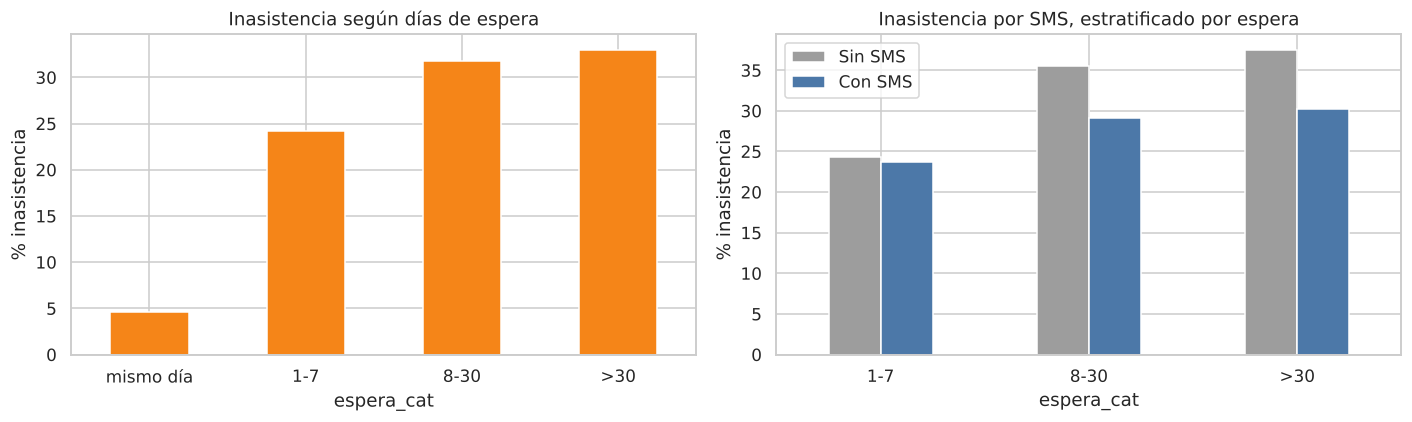
\includegraphics[width=0.92\textwidth]{fig_espera_sms.png}
\caption{Inasistencia según los días de espera y efecto del SMS estratificado por espera.}
\label{fig:sms}
\end{figure}

\subsection{Clasificación de la inasistencia}

\begin{table}[H]
\centering\small
\caption{Desempeño de los clasificadores. Umbral elegido en validación para maximizar el F1.}
\label{tab:clf}
\begin{tabular}{lrrrrrr}
\toprule
& \multicolumn{2}{c}{Validación} & \multicolumn{4}{c}{Prueba} \\
\cmidrule(lr){2-3}\cmidrule(lr){4-7}
Modelo & AUC-ROC & Brecha AUC\textsuperscript{a} & AUC-ROC & F1 & Recall & Precisión \\
\midrule
XGBoost & 0,747 & 0,031 & \textbf{0,740} & 0,455 & 0,770 & 0,323 \\
Random Forest & 0,745 & 0,047 & 0,739 & 0,455 & 0,735 & 0,330 \\
MLP (PyTorch) & 0,745 & 0,008 & 0,738 & 0,454 & 0,756 & 0,324 \\
Logística (referencia) & 0,733 & 0,001 & 0,729 & 0,451 & 0,806 & 0,313 \\
\bottomrule
\multicolumn{7}{l}{\footnotesize \textsuperscript{a} AUC en entrenamiento menos AUC en validación.}
\end{tabular}
\end{table}

Los tres modelos avanzados superan a la referencia en AUC-ROC y F1, en validación y en prueba, con lo cual se cumple el primer objetivo específico. La ganancia es de alrededor de 0,01 de AUC (Tabla~\ref{tab:clf}). XGBoost se eligió por tener el mejor AUC en validación y en prueba con una brecha de sobreajuste menor que la de Random Forest. Con un umbral de 0,52, en prueba detecta 2.578 de las 3.349 inasistencias, a cambio de 5.394 falsas alarmas. El MLP se detuvo en la época 32 y restauró los pesos de la época 28; su pérdida de validación queda por debajo de la de entrenamiento porque el \emph{dropout} solo actúa al entrenar (Figura~\ref{fig:mlp}).

\begin{figure}[H]
\centering
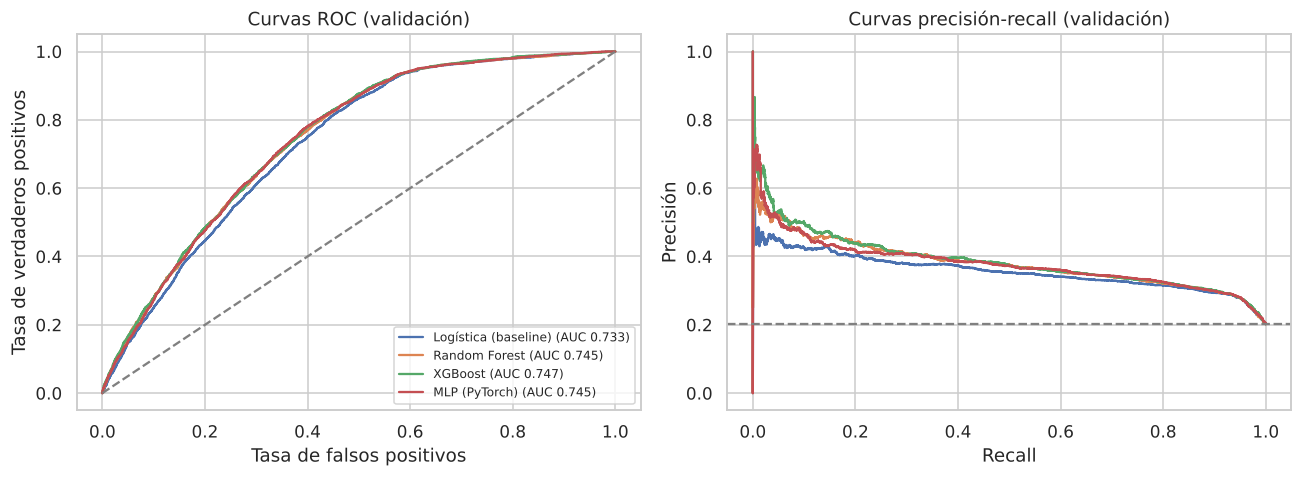
\includegraphics[width=0.92\textwidth]{roc_pr.png}
\caption{Curvas ROC y de precisión-recall en validación.}
\end{figure}

\begin{figure}[H]
\centering
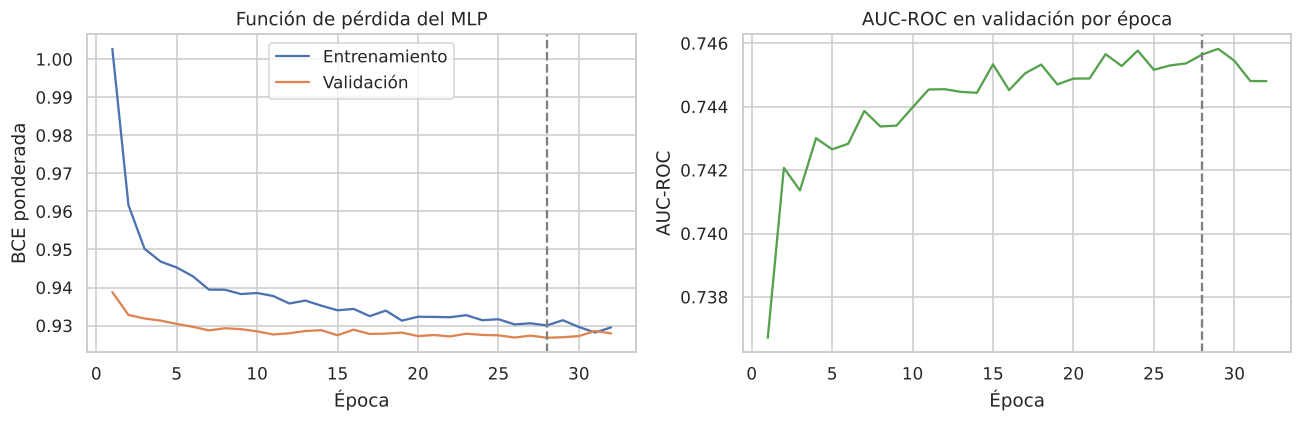
\includegraphics[width=0.85\textwidth]{mlp_perdida.png}
\caption{Función de pérdida y AUC-ROC del MLP por época. La línea punteada marca la mejor época.}
\label{fig:mlp}
\end{figure}

\textbf{Interpretabilidad.} En el análisis SHAP (Figura~\ref{fig:shap}) los días de espera son la variable de mayor peso, seguidos del indicador de cita del mismo día, la edad, el número de citas en la misma fecha y el barrio. Esperas largas, menor edad y un historial de inasistencias empujan la predicción hacia la inasistencia. El SMS aparece con valores SHAP negativos: una vez el modelo conoce la espera, haber recibido el recordatorio reduce el riesgo estimado, lo que coincide con el análisis estratificado.

\begin{figure}[H]
\centering
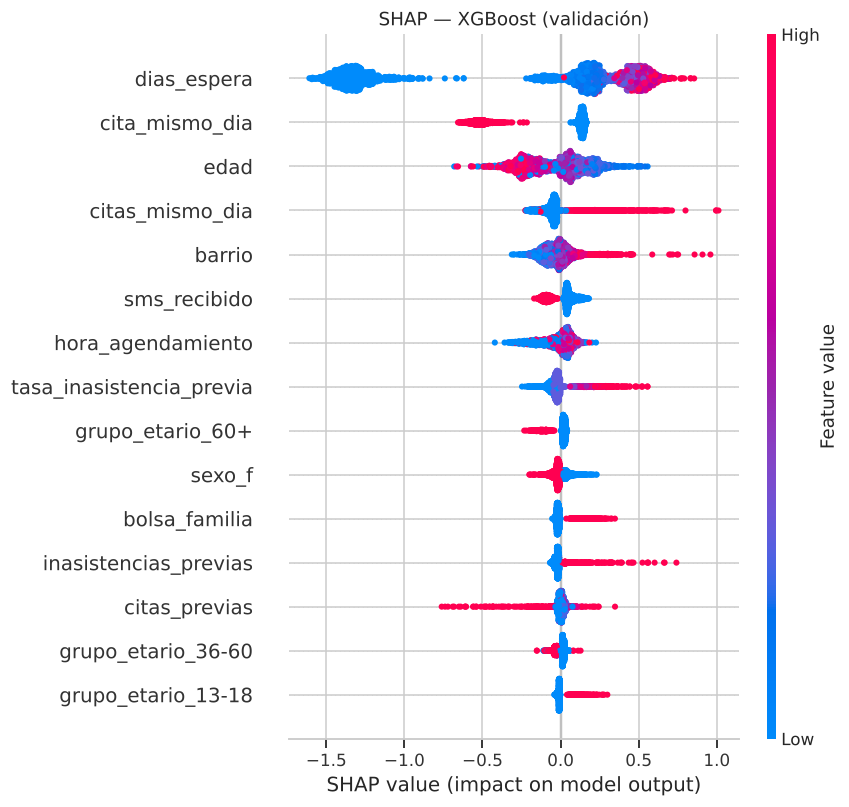
\includegraphics[width=0.62\textwidth]{shap.png}
\caption{Valores SHAP del clasificador XGBoost sobre 3.000 citas de validación.}
\label{fig:shap}
\end{figure}

\subsection{Regresión de los días de espera}

\begin{table}[H]
\centering\small
\caption{Desempeño de los modelos de regresión de los días de espera.}
\label{tab:reg}
\begin{tabular}{lrrrr}
\toprule
& Validación & \multicolumn{3}{c}{Prueba} \\
\cmidrule(lr){2-2}\cmidrule(lr){3-5}
Modelo & $R^2$ & $R^2$ & RMSE (días) & MAE (días) \\
\midrule
XGBoost Regressor & 0,131 & \textbf{0,138} & 14,07 & 10,05 \\
ElasticNet & 0,079 & 0,077 & 14,57 & 10,53 \\
Lineal múltiple (referencia) & 0,079 & 0,077 & 14,57 & 10,53 \\
\bottomrule
\end{tabular}
\end{table}

XGBoost casi duplica el $R^2$ del modelo lineal, pero el error absoluto medio sigue siendo de unos 10 días (Tabla~\ref{tab:reg}). ElasticNet no mejora a la regresión lineal: la regularización elegida es débil (\texttt{alpha} $\approx$ 0,015), lo que indica que el problema no es de sobreajuste sino de falta de información. El barrio es la variable más importante del regresor. La diferencia de $R^2$ entre entrenamiento (0,185) y validación (0,131) muestra un sobreajuste moderado.

\subsection{Segmentación de pacientes}
La silueta más alta se obtuvo con K = 2 (0,370), pero esa partición solo separa a quienes faltaron (tasa media de 0,80) de quienes asistieron (0,02) y repite la variable objetivo. Entre K $\geq$ 3, el valor con mayor silueta antes de que la inercia deje de bajar al menos 10\,\% fue K = 5 (silueta de 0,349). El clustering jerárquico de Ward obtuvo una silueta de 0,327 y un índice de Rand ajustado de 0,65 frente a K-Means, lo que indica segmentos estables entre métodos.

\begin{table}[H]
\centering\small
\caption{Perfil de los segmentos de pacientes (K-Means, K = 5).}
\label{tab:seg}
\begin{tabular}{p{4.6cm}rrrrrr}
\toprule
Segmento & \% pac. & Edad & Citas & Espera (días) & \% SMS & Inasist. citas \\
\midrule
Citas cercanas, asistieron & 33,2 & 28,9 & 1,2 & 5,1 & 0,9 & 0,0\,\% \\
Usuarios frecuentes & 21,3 & 33,8 & 3,7 & 10,1 & 34,5 & 25,1\,\% \\
Espera larga con SMS, asistieron & 18,9 & 37,5 & 1,3 & 20,4 & 91,4 & 0,0\,\% \\
Adultos mayores con condiciones crónicas & 13,6 & 62,4 & 1,5 & 7,4 & 15,9 & 4,9\,\% \\
Espera larga, no asistieron & 13,0 & 33,2 & 1,1 & 18,8 & 45,7 & 100,0\,\% \\
\bottomrule
\end{tabular}
\end{table}

\begin{figure}[H]
\centering
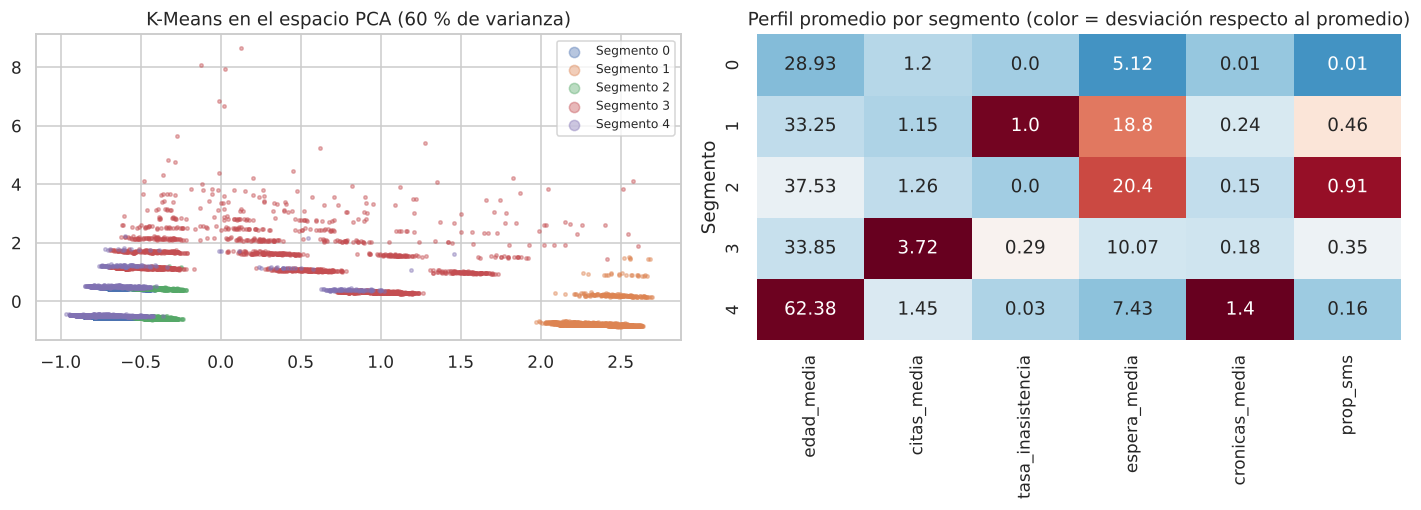
\includegraphics[width=\textwidth]{segmentos.png}
\caption{Segmentos en el espacio de las dos primeras componentes principales y perfil promedio por segmento.}
\end{figure}

\subsection{Tablero interactivo}
El tablero se construyó con Streamlit y se desplegó en Streamlit Community Cloud (\pend{URL del tablero}). Incluye filtros por fecha, sexo, edad, días de espera, SMS, barrio y segmento; tarjetas con el número de citas, la tasa de inasistencia, la espera media, la cobertura de SMS y el AUC del modelo; un módulo de predicción en vivo que entrega la probabilidad de inasistencia, un nivel de riesgo con la acción de recordatorio sugerida y la espera estimada para el perfil; y un módulo de segmentación con el mapa interactivo de clústeres y sus perfiles (Figura~\ref{fig:tablero}). Para no depender de archivos binarios de una versión concreta de las librerías, el tablero vuelve a entrenar los modelos al iniciar con los hiperparámetros elegidos en la Fase 3 y reproduce las mismas métricas de prueba.

\begin{figure}[H]
\centering
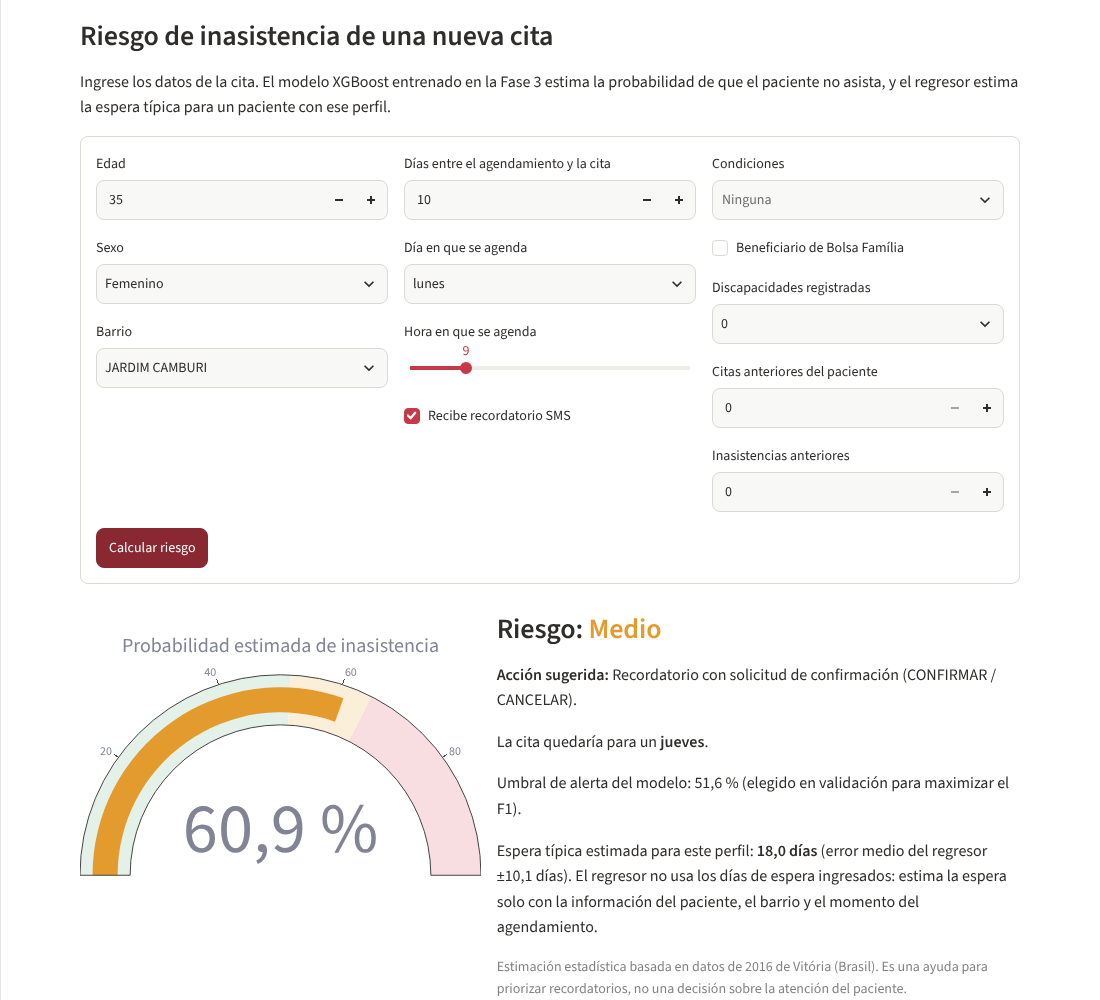
\includegraphics[width=0.75\textwidth]{tablero_prediccion.png}
\caption{Módulo de predicción en vivo del tablero.}
\label{fig:tablero}
\end{figure}

\section{Discusión}

\textbf{Respuesta a las preguntas de investigación.} Los días de espera son el principal predictor de la inasistencia, seguidos de la edad, el historial del paciente y el barrio. La relación entre espera e inasistencia se mantiene al controlar por el SMS, y el SMS se asocia con menor inasistencia solo cuando se compara dentro de un mismo tramo de espera, tanto en el análisis estratificado como en los valores SHAP. Las variables disponibles explican poco de la espera ($R^2$ de 0,138): el barrio, como aproximación de la unidad de atención, es lo que más aporta. En cuanto a perfiles, se distinguen pacientes con citas cercanas, usuarios frecuentes con inasistencia intermitente, adultos mayores con condiciones crónicas y alta adherencia, y dos grupos con espera larga que se diferencian por la cobertura de SMS y por el resultado.

\textbf{Desempeño de los modelos.} Que tres algoritmos tan distintos (bosques aleatorios, \emph{gradient boosting} y una red neuronal) lleguen al mismo AUC de alrededor de 0,74 y que la regresión logística quede a solo 0,01 sugiere que el límite está en la información del dataset y no en el modelo. Salazar et al. (2022) reportaron un AUC de 0,969 con Random Forest, pero sobre datos propios de un centro de rehabilitación que incluían el contacto previo con el paciente y el mes de la cita, por lo que los resultados no son comparables con los de este trabajo. Un AUC de 0,74 no sirve para decisiones individuales de alto impacto, pero sí para ordenar a quién recordar primero, donde el costo de un falso positivo es un mensaje adicional.

\textbf{Implicaciones para AgendamientoIA.} Los resultados sugieren tres reglas para la política de recordatorios: priorizar las citas con espera larga, en especial las de más de una semana; aumentar la intensidad del recordatorio (confirmación explícita CONFIRMAR / CANCELAR) en pacientes con inasistencias previas; y, en las citas de mayor riesgo, ofrecer una fecha más cercana o liberar el cupo para la lista de espera. El tablero implementa estas reglas en el módulo de predicción como acción sugerida.

\textbf{Limitaciones.} Los datos cubren seis semanas de citas en una ciudad brasileña en 2016, y el sistema de salud y los hábitos de comunicación pueden diferir de los colombianos actuales; la transferencia debe validarse con datos del piloto. El dataset no incluye especialidad, profesional, canal de agendamiento ni el contenido o el momento del SMS. El envío de SMS no fue aleatorio, así que su efecto es una asociación y no una relación causal. Los segmentos incluyen la tasa de inasistencia histórica y, por tanto, describen la población de forma retrospectiva; no deben usarse como predictor de una cita futura. Por último, el modelo usa variables como el barrio y la condición socioeconómica, que en un despliegue real exigen revisar que la priorización no reduzca el acceso de grupos vulnerables: el riesgo alto debe traducirse en más apoyo al paciente, no en menos oportunidades de cita.

\section{Conclusiones y trabajo futuro}

El proyecto recorrió el ciclo completo de ciencia de datos sobre un conjunto público de 110.527 citas. Las decisiones de la Fase 2 (partición agrupada por paciente, preprocesamiento dentro de \emph{pipelines} y exclusión de variables que revelan el objetivo) permitieron obtener métricas que se sostienen en un conjunto de prueba no usado durante el desarrollo. XGBoost alcanzó un AUC-ROC de 0,740 y detectó el 77\,\% de las inasistencias, con lo que se cumple el objetivo de clasificación. La regresión de la espera mostró que las variables del paciente no bastan para estimarla, un resultado útil en sí mismo: la espera depende de la oferta de agenda. La segmentación produjo cinco perfiles interpretables y aportó, junto con SHAP, evidencia observacional de que el recordatorio se asocia con mayor asistencia en las citas lejanas.

Como trabajo futuro se proponen: (1) reentrenar y validar el modelo con los registros del piloto de AgendamientoIA, que incluyen especialidad, EPS y la respuesta del paciente al recordatorio por WhatsApp; (2) diseñar un experimento controlado sobre la intensidad y el momento del recordatorio para estimar su efecto causal; (3) incorporar variables de oferta para mejorar la estimación de la espera; y (4) evaluar la equidad del modelo por grupo de edad, sexo y condición socioeconómica antes de cualquier uso operativo.

\textbf{Repositorio y reproducibilidad.} El código, los cuadernos de las cuatro fases, el tablero y el archivo \texttt{requirements.txt} con las versiones exactas están en \pend{URL del repositorio en GitHub}.

\section*{Referencias}
\setlength{\parindent}{-1.27cm}\setlength{\leftskip}{1.27cm}

Dantas, L. F., Fleck, J. L., Cyrino Oliveira, F. L., \& Hamacher, S. (2018). No-shows in appointment scheduling: A systematic literature review. \emph{Health Policy, 122}(4), 412--421. \url{https://doi.org/10.1016/j.healthpol.2018.02.002}

Hoppen, J. (2016). \emph{Medical appointment no shows} [Conjunto de datos]. Kaggle. \url{https://www.kaggle.com/datasets/joniarroba/noshowappointments}

Lundberg, S. M., \& Lee, S.-I. (2017). A unified approach to interpreting model predictions. En \emph{Advances in Neural Information Processing Systems 30} (pp. 4765--4774).

Manarte, P., \& Guedes, J. (2024). Technology and access to healthcare with different scheduling systems: A scoping review. \emph{Healthcare Informatics Research}.

Ministerio de Salud y Protección Social. (2013). \emph{Resolución 1552 de 2013}. República de Colombia.

Salazar, L. H. A., Leithardt, V. R. Q., Parreira, W. D., Fernandes, A. M. da R., Barbosa, J. L. V., \& Correia, S. D. (2022). Application of machine learning techniques to predict a patient's no-show in the healthcare sector. \emph{Future Internet, 14}(1), Artículo 3. \url{https://doi.org/10.3390/fi14010003}

Van Buchem, M. M., et al. (2022). Artificial intelligence for patient scheduling in the real-world health care setting: A metanarrative review. \emph{Health Informatics Journal}.

\end{document}
